\documentclass[11pt]{article}
\usepackage{lipsum}
\usepackage{charsheet}

\usepackage{pgfkeys}



\newsectionenv[]{magic}{MAGIC}
  {\begin{minipage}[t][87mm][t]{\hsize}}
  {\end{minipage}}
\newsectionenv{attacks}{ATTACKS}{}{}
\newsectionenv{features}{CLASS FEATURES}{}{}
\newsectionenv[width=74mm,decorated clipped rectangle]{equipment}{EQUIPMENT}
   {\medskip
    \small
     \begin{eqlist}}
   {\end{eqlist}}


\newsectionenv[width=38mm]{proficiencies}{PROFICIENCIES}
   {\medskip
    \begin{minipage}[t][138mm][t]{\hsize}
     \begin{proflist}}
   {\end{proflist}
    \end{minipage}}

  

\begin{document}


\newcommand\nextstatloc{inside north west corner=of stats background}



%\makeatletter
%\newcommand{\stat@starred}[2]{%
%  \newcounter{tempmodifier}%
%  \newcounter{tempmodifierwithprof}%
%  \setcounter{tempmodifier}{(#2 - 10) / 2}%
%  \setcounter{tempmodifierwithprof}{\value{tempmodifier} + \value{proficiencybonus}}%
%  \fullstatbox[\nextstatloc]{#1}{#2}{\thetempmodifier}{\thetempmodifierwithprof}%
%}
%\newcommand{\stat@}{\@ifstar{\stat@starred}{\stat}}
%\let\stat\stat@
%\makeatother


\noindent
\begin{charsheet}

  \input{barb}
%  \setcounter{proficiency bonus}{2}

  \node [dndfull,height=20mm,fill=playername,below=of top] (splash) 
     {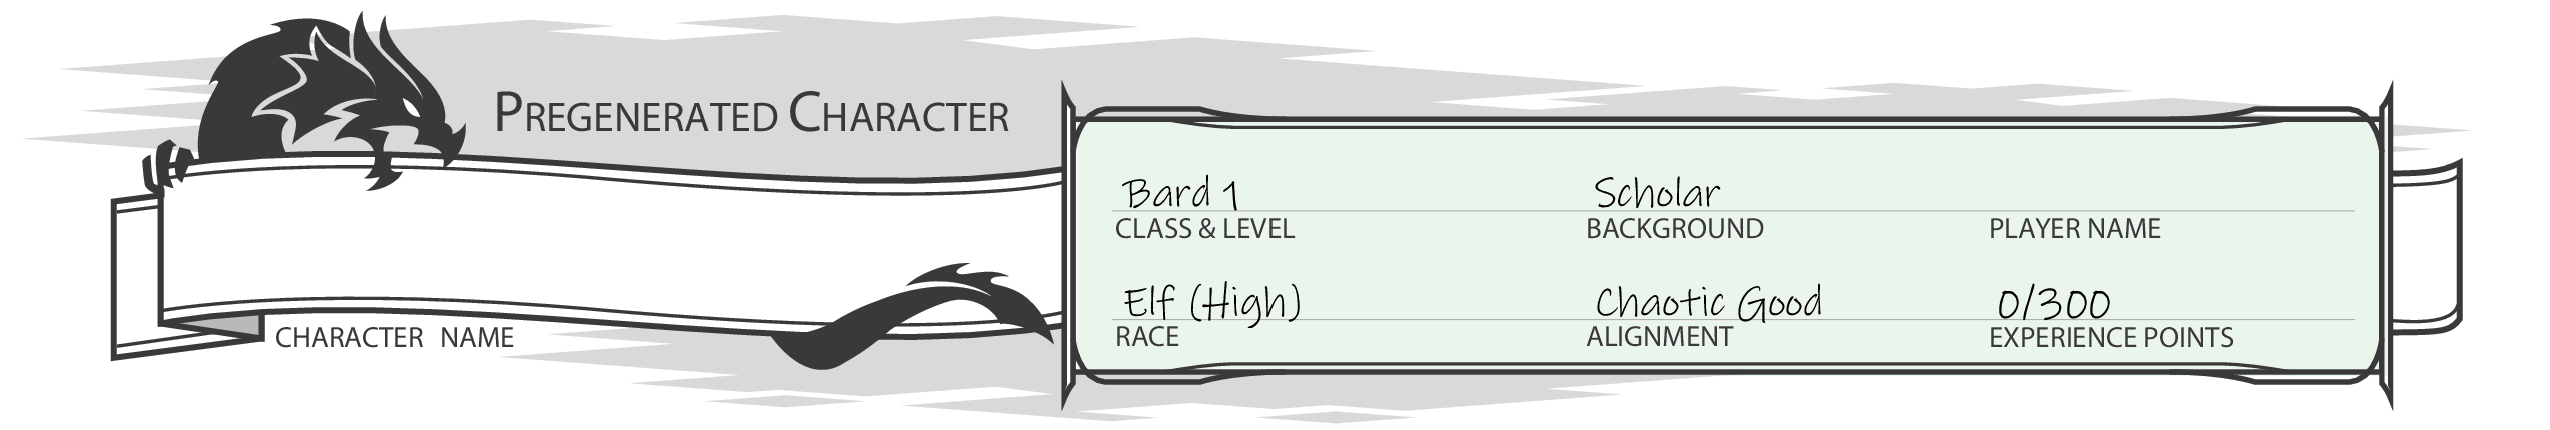
\includegraphics[width=\textwidth]{splash.png}};

  \begingroup\sffamily

  
  
  \node (class and level)
    [fill=splashfield,anchor=south west,width=38mm] at ($(splash.south west)+(88mm,19mm)$)
    {\hbox to 36mm{\itshape \getDND*{CLASS + LEVEL}\hfill}}
    ;

  \node[fill=splashfield,right=1mm of class and level,width=36mm]
    {\hbox to 36mm{\itshape \getDND*{BACKGROUND}\hfill}}
    ;
    
  \node (race) [fill=splashfield,below left corner=4.2mm of class and level,width=36mm]
    {\hbox to 36mm{\itshape \getDND*{RACE}\hfill}}
    ;
    
  \node (alignment) [fill=splashfield,right=1mm of race,width=26mm]
    {\hbox to 26mm{\itshape \getDND*{ALIGNMENT}\hfill}}
    ;
    
  \node (alignment) [fill=splashfield,right=1mm of alignment,width=26mm]
    {\hbox to 26mm{\itshape \getDND*{EXPERIENCE POINTS}\hfill}}
    ;
    

\Large

      \node (hpbackground) 
        [outer sep=0pt,fill=hpetc,below right corner=of splash,width=102mm, minimum height=46mm] 
       { };

      \node (hitdice)
             [dndhits,width=20mm,inside south east corner=of hpbackground,
             dndlabel=HIT DICE] 
         { \Large \getDND*{HIT DICE}{} }
         ;

      \node (curhp)
            [dndhits,fill=white,width=72mm,left=of hitdice,
             dnd/label={CURRENT HIT POINTS}] 
         { }
         ;

      \node [dndmaxhp,above left corner=of curhp,dndlabel=MAX HP] 
         (maxhp)
         { \Large \getDND*{MAX HP} }
         ;

      \node (initiative)
            [dndmaxhp,right=of maxhp,dndlabel=INITIATIVE] 
         { \getDND*{INITIATIVE} }
         ;

      \node (speed)
            [dndmaxhp,right=of initiative,dndlabel=SPEED] 
         { \getDND*{SPEED} }
         ;


       \node (ac) [dndmaxhp,shield,innershield,draw,ultra thick,right=of speed,width=15mm,
                   dndlabel={\noexpand\tinystacklabel{ARMOR}{CLASS}},
            ]
      {\raisebox{4mm}{\getDND*{ARMOR CLASS}}}
      ;

  \endgroup


\begin{attacks}[below right corner=of hpbackground]{}
    \centering
    \begin{attackstab}
    Shortsword & +4 & 1d6+2 & piercing & 5 ft. & ---\\
    Hand Axe (off~hand) [B]& +5 & 1d6 & slashing & 5~ft or 20/60~ft& ---\\
    \end{attackstab}
\end{attacks}


% \node (attacks) at (hpbackground.south west) {A};

\ifDNDdefined{MAGIC}
{
\begin{magic}[below=of attacks]{}
\centering
\begin{featurestab}
% Magic section (right side, middle)
  \textsf{CANTRIPS}\\
  Friends& Does a thing\\
  Ray of Frost& asdf\\
  \multicolumn2{l}{\textsf{1st-LEVEL SPELLS \spellslots{3}}}\\
\end{featurestab}
\end{magic}
}
{\node (magic) at (attacks.south) {};}

\ifDNDdefined{FEATURES}{
\begin{features}[below=of magic]{}
\let\described=\feature
\begin{featurestab}
\getDND{FEATURES}
\end{featurestab}
\end{features}
}{}

\node (stats background) 
      [fill=stats,width=24mm,height=163mm,below left corner=of splash] { };

\dndstat{STRENGTH}{STR}
\dndstat{DEXTERITY}{DEX}
\dndstat{CONSTITUTION}{CON}
\dndstat{INTELLIGENCE}{INT}
\dndstat{WISDOM}{WIS}
\dndstat{CHARISMA}{CHA}

  
\begin{equipment}[left of lower corner=of features]
    \item Clothes (Fine)
    \item Leather Armor
    \item Shortsword
    \item Lyre
    \item Backpack
    \item Bedroll, Book of Elvish Poetry
    \item Bottle of Ink, Ink Pen
    \item Parchment (10 sheets), Tinderbox
    \item Trail Rations (10 days), Waterskin
\end{equipment}

\path (equipment.north west) +(3mm,-4mm) coordinate (coin top left);


\coin{cp}{Cu}{10}
\coin{sp}{Ag}{5}
\coin{gp}{Au}{G}
  
\node (proficiency bonus)
      [proficiencies,decorated stub rectangle,width=38.001mm,height=8mm,
       right of upper corner=3.5mm of stats background]
   {\hbox to 0pt{\hss\hspace*{9mm}\tiny\textsf{PROFICIENCY BONUS}\hss}}
   ;
\node [anchor=west,proficiencies,circle,
       width=10mm,height=10mm,line width=1.5pt,draw]
       at ($(proficiency bonus.west)+(-2mm,0mm)$)
      {\large\textsf{+\arabic{proficiency bonus}}};

% Proficiencies section (middle top)
\begin{proficiencies}[below=of proficiency bonus,width=38.002mm]
  \small
\item
  {Acrobatics}
\item
  Arcana
\item
  History
\item
  Investigation
\item
  Perception
\item
  Performance
\item
  Persuasion
\item
  Musical Instrument (Lyre)
\item
  Language (Common)
\item
  Language (Elvish)
\end{proficiencies}

\node (passive perception)
   [dndmaxhp,left=10mm of maxhp,width=24mm] 
   {\Large\textsf{13}}
   ;

\dndlabel{passive perception}{\pplabel}

\node (senses)
   [dndmaxhp,left=10mm of curhp,width=24mm] 
%   {\itshape\begin{tabular}{c}{Darkvision}\\{60~ft}\\[3pt]\end{tabular}}
   {\parbox{20mm}{\centering\itshape\getDND*{SENSES}}}
   ;
\dndlabel{senses}{\scriptsize SENSES}


\end{charsheet}




\end{document}
